\begin{figure}
\centering
\begin{tikzpicture}
  \node (input) {
    \begin{tikzpicture}
      \node[inner sep=0pt] (circuit) {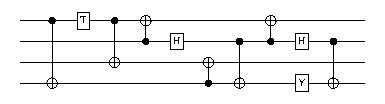
\includegraphics[scale=2]{Figures/circuits/interesting}};  
      \node[above left=8mm and -7mm of circuit.west, opacity=0.9] {\footnotesize \(A\)};
      \node[above left=1mm and -7mm of circuit.west, opacity=0.9] {\footnotesize \(B\)};
      \node[below left=1mm and -7mm of circuit.west, opacity=0.9] {\footnotesize \(C\)};
      \node[below left=8mm and -7mm of circuit.west, opacity=0.9] {\footnotesize \(D\)};
      \node[below right=4.3mm and 12.8mm of circuit.west, opacity=0.9] {\footnotesize \(\alpha\)};
      \node[right=0.8mm and 34.4mm of circuit.west, opacity=0.9] {\footnotesize \(\beta\)};
      \node[above right=4.3mm and 44.7mm of circuit.west, opacity=0.9] {\footnotesize \(\gamma\)};
      \node[below right=4.3mm and 65.8mm of circuit.west, opacity=0.9] {\footnotesize \(\delta\)};
      \node[below right=4.3mm and 76.4mm of circuit.west, opacity=0.9] {\footnotesize \(\eta\)};
      \node[above right=4.3mm and 87.0mm of circuit.west, opacity=0.9] {\footnotesize \(\theta\)};
      \node[below right=4.3mm and 108.4mm of circuit.west, opacity=0.9] {\footnotesize \(\mu\)};
      \node[right=-3mm of circuit.north west, font=\itshape] (text) {Input:};
    \end{tikzpicture}
  };
  \node[below=5mm of input] (pulled) {
    \begin{tikzpicture}
      \node[inner sep=0pt] (circuit) {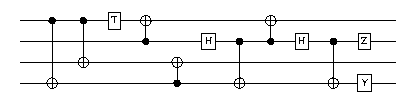
\includegraphics[scale=2]{Figures/circuits/interestingPulled}};  
      \node[above left=8mm and -7mm of circuit.west, opacity=0.9] {\footnotesize \(A\)};
      \node[above left=1mm and -7mm of circuit.west, opacity=0.9] {\footnotesize \(B\)};
      \node[below left=1mm and -7mm of circuit.west, opacity=0.9] {\footnotesize \(C\)};
      \node[below left=8mm and -7mm of circuit.west, opacity=0.9] {\footnotesize \(D\)};
      \node[below right=4.3mm and 12.8mm of circuit.west, opacity=0.9] {\footnotesize \(\alpha\)};
      \node[right=0.8mm and 24.2mm of circuit.west, opacity=0.9] {\footnotesize \(\beta\)};
      \node[above right=4.3mm and 44.7mm of circuit.west, opacity=0.9] {\footnotesize \(\gamma\)};
      \node[below right=4.3mm and 56.1mm of circuit.west, opacity=0.9] {\footnotesize \(\delta\)};
      \node[below right=4.3mm and 76.4mm of circuit.west, opacity=0.9] {\footnotesize \(\eta\)};
      \node[above right=4.3mm and 87.0mm of circuit.west, opacity=0.9] {\footnotesize \(\theta\)};
      \node[below right=4.3mm and 108.4mm of circuit.west, opacity=0.9] {\footnotesize \(\mu\)};
      \node[right=-3mm of circuit.north west, font=\itshape] (text) {After preprocessing (\texttt{SlideCNOTs} extension):};
    \end{tikzpicture}
  };
  \node[below left=5mm and -60mm of pulled] (FF) {
    \begin{tikzpicture}
      \coordinate (A) at (135:22mm);
      \coordinate (B) at (45:22mm);
      \coordinate (C) at (225:22mm);
      \coordinate (D) at (315:22mm);
      \coordinate[below left=12mm and 12mm of B] (auxB);
      \draw (C) -- (A);
      \draw (A) edge[out=290,in=160] (D);
      \draw (B) -- (auxB);
      \draw (A) -- (auxB);
      \draw (D) -- (auxB);
      \draw (A) -- (B);
      \draw (D) -- (B);
      \draw (C) -- (D);
      \node[circle, right=-2.5mm of A, fill=white, inner sep=0pt, minimum size=5mm] {\(A\)};
      \node[circle, right=-2.5mm of B, fill=white, inner sep=0pt, minimum size=5mm] {\(B\)};
      \node[circle, right=-2.5mm of C, fill=white, inner sep=0pt, minimum size=5mm] {\(C\)};
      \node[circle, right=-2.5mm of D, fill=white, inner sep=0pt, minimum size=5mm] {\(D\)};
      \coordinate[below left=20mm and 4mm of A] (p0);
      \coordinate[below right=20mm and 4mm of B] (p1);
      \pic (cut) {cut=p0/p1};
      \node[above left=0mm and 8mm of A, font=\itshape] (text) {a)};
    \end{tikzpicture}
  };
  \node[right=15mm of FF] (FT) {
    \begin{tikzpicture}
      \coordinate (A) at (135:22mm);
      \coordinate (B) at (45:22mm);
      \coordinate (C) at (225:22mm);
      \coordinate (D) at (315:22mm);
      \coordinate (a) at (270:7mm);
      \coordinate (b) at (180:18mm);
      \coordinate (c) at (90:18mm);
      \coordinate (d) at (270:18mm);
      \coordinate (e) at (30:7mm);
      \coordinate (t) at (150:7mm);
      \coordinate (m) at (0:18mm);
      \coordinate[above left=5mm and 1mm of t] (auxAt);
      \coordinate[above right=7mm and 1mm of e] (auxB);
      \coordinate[above right=5mm and 5mm of C] (auxC);
      \draw (A) edge[out=290,in=145] (a);
      \draw (b) -- (A);
      \draw[ultra thick] (A) -- (auxAt);
      \draw[ultra thick] (t) -- (auxAt);
      \draw[ultra thick] (c) -- (auxAt);
      \draw (B) -- (auxB);
      \draw (t) -- (auxB);
      \draw (e) -- (auxB);
      \draw[ultra thick] (C) -- (auxC);
      \draw[ultra thick] (b) -- (auxC);
      \draw[ultra thick] (d) -- (auxC);
      \draw[ultra thick] (D) -- (e);
      \draw[ultra thick] (m) -- (D);
      \draw (c) -- (B);
      \draw (m) -- (B);
      \draw[ultra thick] (a) -- (D);
      \draw (d) -- (D);
      \node[circle, right=-2.5mm of A, fill=white, inner sep=0pt, minimum size=5mm] {\(A\)};
      \node[circle, right=-2.5mm of B, fill=white, inner sep=0pt, minimum size=5mm] {\(B\)};
      \node[circle, right=-2.5mm of C, fill=white, inner sep=0pt, minimum size=5mm] {\(C\)};
      \node[circle, right=-2.5mm of D, fill=white, inner sep=0pt, minimum size=5mm] {\(D\)};
      \node[circle, right=-2.5mm of a, fill=white, inner sep=0pt, minimum size=5mm] {\(\alpha\)};
      \node[circle, right=-2.5mm of b, fill=white, inner sep=0pt, minimum size=5mm] {\(\beta\)};
      \node[circle, right=-2.5mm of c, fill=white, inner sep=0pt, minimum size=5mm] {\(\gamma\)};
      \node[circle, right=-2.5mm of d, fill=white, inner sep=0pt, minimum size=5mm] {\(\delta\)};
      \node[circle, right=-2.5mm of e, fill=white, inner sep=0pt, minimum size=5mm] {\(\eta\)};
      \node[circle, right=-2.5mm of t, fill=white, inner sep=0pt, minimum size=5mm] {\(\theta\)};
      \node[circle, right=-2.5mm of m, fill=white, inner sep=0pt, minimum size=5mm] {\(\mu\)};
      \coordinate[above right=4mm and 6.5mm of A] (p0);
      \coordinate[below right=4mm and 6.5mm of C] (p1);
      \pic (cut) {cut=p0/p1};
      %\draw[dash pattern={on 7pt off 2pt on 1pt off 2pt}, line width=1pt, opacity=0.65] (p1) edge[out=0,in=150,looseness=0.7] (p2);
      \node[above left=0mm and 8mm of A, font=\itshape] (text) {b)};
    \end{tikzpicture}
  };
  \node[below=5mm of FF] (TF) {
    \begin{tikzpicture}
      \coordinate (A) at (135:22mm);
      \coordinate (B) at (45:22mm);
      \coordinate (C) at (225:22mm);
      \coordinate (D) at (315:22mm);
      \coordinate[above right=10mm and 10mm of C] (auxAc);
      \coordinate[below left=10mm and 10mm of B] (auxB);
      \draw (A) -- (auxAc);
      \draw (D) -- (auxAc);
      \draw (C) -- (auxAc);
      \draw (B) -- (auxB);
      \draw (A) -- (auxB);
      \draw (D) -- (auxB);
      \draw (A) -- (B);
      \draw (D) -- (B);
      \draw (C) -- (D);
      \node[circle, right=-2.5mm of A, fill=white, inner sep=0pt, minimum size=5mm] {\(A\)};
      \node[circle, right=-2.5mm of B, fill=white, inner sep=0pt, minimum size=5mm] {\(B\)};
      \node[circle, right=-2.5mm of C, fill=white, inner sep=0pt, minimum size=5mm] {\(C\)};
      \node[circle, right=-2.5mm of D, fill=white, inner sep=0pt, minimum size=5mm] {\(D\)};
      \coordinate[below left=10mm and 4mm of A] (p0);
      \coordinate[above right=10mm and 4mm of D] (p1);
      \pic (cut) {cut=p0/p1};
      \node[above left=0mm and 8mm of A, font=\itshape] (text) {c)};
    \end{tikzpicture}
  };
  \node[right=15mm of TF] (TT) {
    \begin{tikzpicture}
      \coordinate (A) at (135:22mm);
      \coordinate (B) at (45:22mm);
      \coordinate (C) at (225:22mm);
      \coordinate (D) at (315:22mm);
      \coordinate (a) at (270:7mm);
      \coordinate (b) at (180:18mm);
      \coordinate (c) at (90:18mm);
      \coordinate (d) at (270:18mm);
      \coordinate (e) at (30:7mm);
      \coordinate (t) at (150:7mm);
      \coordinate (m) at (0:18mm);
      \coordinate[below right=2mm and 9mm of b] (auxAc);
      \coordinate[above left=5mm and 1mm of t] (auxAt);
      \coordinate[above right=7mm and 1mm of e] (auxB);
      \coordinate[above right=5mm and 5mm of C] (auxC);
      \coordinate[below left=5mm and 5mm of m] (auxD);
      \draw (A) -- (auxAc);
      \draw (a) -- (auxAc);
      \draw (b) -- (auxAc);
      \draw[ultra thick] (A) -- (auxAt);
      \draw[ultra thick] (t) -- (auxAt);
      \draw[ultra thick] (c) -- (auxAt);
      \draw (B) -- (auxB);
      \draw (t) -- (auxB);
      \draw (e) -- (auxB);
      \draw[ultra thick] (C) -- (auxC);
      \draw[ultra thick] (b) -- (auxC);
      \draw[ultra thick] (d) -- (auxC);
      \draw[ultra thick] (D) -- (auxD);
      \draw[ultra thick] (e) -- (auxD);
      \draw[ultra thick] (m) -- (auxD);
      \draw (c) -- (B);
      \draw (m) -- (B);
      \draw[ultra thick] (a) -- (D);
      \draw (d) -- (D);
      \node[circle, right=-2.5mm of A, fill=white, inner sep=0pt, minimum size=5mm] {\(A\)};
      \node[circle, right=-2.5mm of B, fill=white, inner sep=0pt, minimum size=5mm] {\(B\)};
      \node[circle, right=-2.5mm of C, fill=white, inner sep=0pt, minimum size=5mm] {\(C\)};
      \node[circle, right=-2.5mm of D, fill=white, inner sep=0pt, minimum size=5mm] {\(D\)};
      \node[circle, right=-2.5mm of a, fill=white, inner sep=0pt, minimum size=5mm] {\(\alpha\)};
      \node[circle, right=-2.5mm of b, fill=white, inner sep=0pt, minimum size=5mm] {\(\beta\)};
      \node[circle, right=-2.5mm of c, fill=white, inner sep=0pt, minimum size=5mm] {\(\gamma\)};
      \node[circle, right=-2.5mm of d, fill=white, inner sep=0pt, minimum size=5mm] {\(\delta\)};
      \node[circle, right=-2.5mm of e, fill=white, inner sep=0pt, minimum size=5mm] {\(\eta\)};
      \node[circle, right=-2.5mm of t, fill=white, inner sep=0pt, minimum size=5mm] {\(\theta\)};
      \node[circle, right=-2.5mm of m, fill=white, inner sep=0pt, minimum size=5mm] {\(\mu\)};
      \coordinate[above=7mm of b] (p1);
      \coordinate[below=4mm of t] (p2);
      \coordinate[below=7mm of m] (p3);
      \coordinate[left=4mm of p1] (p0);
      \coordinate[right=4mm of p3] (p4);
      \draw[dash pattern={on 7pt off 2pt on 1pt off 2pt}, line width=1pt, opacity=0.65] (p0) -- (p1);
      \draw[dash pattern={on 7pt off 2pt on 1pt off 2pt}, line width=1pt, opacity=0.65] (p1) edge[out=0,in=150,looseness=0.7] (p2);
      \draw[dash pattern={on 7pt off 2pt on 1pt off 2pt}, line width=1pt, opacity=0.65] (p2) edge[out=330,in=180,looseness=0.7] (p3);
      \draw[dash pattern={on 7pt off 2pt on 1pt off 2pt}, line width=1pt, opacity=0.65] (p3) -- (p4);
      \node[above left=0mm and 8mm of A, font=\itshape] (text) {d)};
    \end{tikzpicture}
  };
\end{tikzpicture}
\vspace*{2mm}
\caption{Different hypergraphs representing the input circuit. \textit{a)} corresponds to no extensions active. \textit{c)} and \textit{d)} use \texttt{SlideCNOTs}. \textit{b)} and \textit{d)} use \texttt{EitherRemote}. For each hypergraph, the optimal \(k=2\) partition (into two QPUs) is shown. The number of ebits required in each case is: \textit{a)} \(4\), \textit{b)} \(3\), \textit{c)} \(3\), \textit{d)} \(2\).}
\label{fig:modes}
\end{figure}